Though the metastable density measurements appear to be one of only a few
diagnositics conducted during the development of the \acs{rpnd}, they only
provide a limited view of what is happening. Other quantities, such as the ions,
electrons, additional excited states, and fields are all evolving with the
metastables. However, these are all closely related and, provided a sufficiently
detailed model, it should be possible to infer some or all of these parameters
during the development of the \acs{rpnd}. The ideal model would solve
equation~\ref{eq:boltzmann}, the Boltzmann equation for each species, over the
entire geometry, for all velocities, for as long as was required to reach
equilibrium.

Unfortunately, these requirements are somewhat problematic. Solutions to the
Boltzmann equation alone are difficult \cite{Lieberman2005}, let alone for the
dozens of species which may be present in the \acs{rpnd}. The spatial
discretization can be estimated as the cube of the largest length scale (the
discharge apparatus length, about 30 cm) divided by the smallest length scale
(on the order of the Debye length, about 20 $\mu$m). This calculation reveals
the need for nearly $2\times10^{12}$ spatial cells. Similar calculations can be
performed for the time scale (from nanoseconds to minutes) and velocity scale
(from thermal to 100s of eV). It quickly becomes apparent that no existing
computer could handle such a simulation.

\section{Model Development}

Therefore, some approximations of the Boltzmann equation were required in order
to obtain a computationally tractable problem. As discussed in
Chapter~\ref{chp:theory}, the most common approach, and the one applied here, is
the use of \emph{moments} of the Boltzmann equation. These moments average out
the velocity dependence of the Boltzmann equation in favor of macroscopic
properties such as particle densities and mean velocities. They are often used
to develop various fluid approximations for plasmas \cite{Chen1984} (e.g.\ the
two fluid model and the magnetohydrodynamic equations). Fluid models have been
tremendously successful in the description of everything from plasma display
panels \cite{Rauf1999b} to interstellar plasmas \cite{Linde1998}.

The use of moments of the Boltzmann equation does introduce some additional
problems. Reaction rates, such as ionization and excitation, are sensitive to
changes in the distribution of particle velocities. This presents a problem when
the velocity dependence has been averaged out, as in the case of the fluid
models. As a result, a distribution function must be assumed or calculated in
order to determine the reaction rates. The Maxwell-Boltzmann and Druyvesteyn
distributions from Chapter~\ref{chp:theory} are often used for this purpose.
However, they require a number of assumptions which are not necessarily true for
most plasmas. In cases where these distributions cannot be applied, approximate
solutions of the Boltzmann equation are often used \cite{Hagelaar2005} which
employ detailed reaction cross sections to obtain more accurate solutions. The
choice of which approach to use is not easy as the \acs{eedf} is rarely known
\emph{a priori}. Consequently, this topic is considered more thoroughly in
section~\ref{sec:dists}.

From another perspective, fluid models include some or all spatial dimensions.
This can lead to simulations that are still computationally demanding depending
on the length scales involved. In some cases, the number of species and
reactions must be limited in to order to speed up the solution process
\cite{Lieberman2005}. For this reason, simulations may only include one or a few
excited states. Careful choices of the excited states and reactions can produce
excellent results, however this approach can prevent detailed comparisons to
spectroscopic data which can can reveal information about the degree of
equilibrium in the plasma and the electron temperatures, both of interest in the
\acs{rpnd}. Therefore, the model developed here makes additional simplifications
in order include additional a large number of excited states and reactions.

As simplifications had already been made to the velocity space, the next logical
approach was a simplification of the geometric dependence of the model. Several
\acs{fiw} studies were found to have successfully applied ``global models'' to
their systems \cite{Aleksandrov2007, Popov2011}. These models eliminate the
spatial dependence of the Boltzmann moments in favor of an assumed spatial
distribution. This allowed the studies to consider a large number of species and
reaction pathways. Following these examples, a decision was made to use a global
model in the simulation of the \acs{rpnd}. The final model tracked a total of 32
different excited states of helium from before the pulse until the return of the
first reflection. Between these possible states a total of 535 different
reaction processes were incorporated including electron-related reactions,
radiative processes, and inter-atomic interactions.

In order to compare the metastable measurements to the global results, it was
necessary to convert the line-integrated densities from
Chapter~\ref{chp:metastables} to volumetric densities, along the path of the
laser. It has been noted that a similar \acs{fiw} \cite{Vasilyak1994} and the
same \acs{rpnd} \cite{Weatherford2012} exhibited radial variations in emission
intensity, electron density, and metastable density. Unfortunately, the cause of
these variations is not clearly understood. It has been suggested that
high-energy electrons from the walls may be responsible \cite{Weatherford2012a}.
However, lacking any empirical, theoretical, or numerical results with which
describe the evolution of the radial profile during the discharge, the
metastable distribution was simply assumed to be uniform. This assumption likely
affects the inferred plasma parameters, however more accurate results are
possible provided time-resolved measurements of the radial metastable density or
an improved understanding of the \acs{rpnd}.

\subsection{Continuity Equation}

Equation~\ref{eq:cont}, the continuity equation, forms the basis for tracking
the populations of the excited states in the plasma. Eliminating the spatial
gradients reduces this to,
\begin{equation}
  \frac{d n_\alpha}{dt} = G_\alpha - L_\alpha,
  \label{eq:zdmcont}
\end{equation}
where $\alpha$ identifies the particle species, $G$ is the gain term, and $L$ is
the loss term. The gain and loss terms represent all possible reactions which
can alter the population of $\alpha$. The model presented incorporates helium
states up to $n=4$, helium ions, and electrons. It should be noted that helium
dimers and impurities were also likely present in the experimental discharge.
However, they were neglected in the case of this model. As observed in
Chapter~\ref{chp:metastables}, the total e-folding time for the metastable decay
was approximately 25 $\mu$s. This indicates that the processes associated with
the dimers and impurities are irrelevant on the sub-microsecond time scale.

There were several possible processes that were considered for inclusion in the
model:
\begin{itemize}
  \singlespacing
  \item electron impact ionization,
  \item electron impact (de)excitation,
  \item atomic impact (de)excitation,
  \item atomic excitation transfer,
  \item dielectronic recombination,
  \item three-body recombination,
  \item radiative decay, and
  \item diffusion.
\end{itemize}
As with the impurities and dimer formation, diffusion occurs on a much longer
time scale, and was subsequently neglected. Three-body recombination in the
volume of the discharge is not important at the estimated temperatures and
densities \cite{Lieberman2005}, therefore this too was neglected. In general,
dielectronic recombination is a rare process \cite{Nahar2010}, however it was
incorporated in early versions of the model and was subsequently retained.
Inter-atomic excitation and de-excitation is not generally considered important
given the low energies of the atoms in discharges.

The remaining processes were found to be the most important for the \acs{rpnd}.
This included electron-impact ionization and excitation which dominated the
short time-scale dynamics. In addition, excitation transfer between atoms was
found to occur at rates relevant to the simulation period \cite{Lieberman2005}.
Likewise, radiative decay occurred fast enough relative to the simulation period
to necessitate inclusion \cite{Kramida2012}.

For these processes, equation~\ref{eq:zdmcont} was rewritten as,
\begin{multline}
  \frac{dN_i}{dt} =   n_e \left[       \sum_{j\neq i} N_j K^e_{j,i}(T_e) 
                                 - N_i \sum_{j\neq i}     K^e_{i,j}(T_e) \right]
                        + \left[       \sum_{j > i}   N_j K^o_{j,i} 
                                 - N_i \sum_{j < i}       K^o_{i,j}      \right] \\
                    + N_g \left[       \sum_{j\neq i} N_j K^a_{j,i} 
                                 - N_i \sum_{j\neq i}     K^a_{i,j}      \right].
  \label{eq:gcont}
\end{multline}
Here, the subscripts of $i$ and $j$ represent different states of helium, $N$ is
the state density, $K$ is a rate coefficient, $T_e$ is the electron temperature,
and $N_g$ is the neutral helium density. The first subscript of the rate
coefficients represents the initial excited state while the second coefficient
represents the final excited state. Therefore, $K_{ij}$ is a rate coeficient for
a process that transfers an atom from state $i$ to state $j$.

The equation is split into three sets of processes, represented by the
superscripts of the rate coefficients: $e$ - electron impact processes, $o$ -
radiative decay, and $a$ - atomic excitation transfer. Therefore, the first
bracketed term on the right hand side contains all the rate coefficients for
electron impact excitation and de-excitation (including ionization). The second
bracketed term contains the rate coefficients for optical transitions in and out
of the excited state. The final bracketed term contains the gains and losses as
a result of excitation transfer caused by collisions with the ground state
(collisions between excited states are relatively rare).

The rate coefficients in equation~\ref{eq:gcont} are compiled from a number of
different sources. The optical transition rates and the energies of each level
were obtained from the NIST Atomic Spectra Database \cite{Kramida2012}. The
excitation transfer rate coefficients came from the studies of Catherinot and
Dubreuil \cite{Catherinot1981, Dubreuil1980}. Coefficients were only available
for the transitions with $\Delta n=0$ and $n=3,4$. No constants were found for
other excitation transfer reactions. The dielectronic recombination rates were
adapted from the work of Nahar \cite{Nahar2010}.

The semi-empirical relations derived by Ralchenko et al. \cite{Ralchenko2008}
were used to calculate the electron (de)excitation and ionization cross sections
for levels through $n=4$. At the time of writing they were the most accurate set
of cross sections available for neutral helium with a quoted accuracy of 10-30\%
for $\Delta S=0$, and $>30$\% for $\Delta S \neq 0$. Only reactions resulting in
an energetically uphill reaction were tabulated. The inverse or superelastic
cross sections were calculated using the principle of detailed balance
\cite{Kunze2009},
\begin{equation}
  \sigma_{ji}(\epsilon) = \frac{\epsilon}{\epsilon - \Delta\epsilon_{ij}}
    \frac{g_j^2}{g_i}\sigma_{ij},
\end{equation}
where $\Delta\epsilon$ is the threshold energy of the $ij$ reaction and $g$ is
the statistical degeneracy of the corresponding state. These cross sections can
be used to calculate the rate coefficients for each reaction using
equation~\ref{eq:rate}. However, this equation requires an appropriate
\acs{eedf} and leads back to the topic of which one is appropriate for the
\acs{rpnd}.

\subsection{Distribution Effects}\label{sec:dists}

Per the discussion of the Boltzmann equation in Chapter~\ref{chp:theory}, there
are two analytic equilibrium solutions: the Maxwell-Boltzmann distribution, and
the Druyvesteyn distribution. However, research by Starikovskaia and
Starikovskii \cite{Starikovskaia2001} has shown that the \acs{eedf} in a
nitrogen \acs{fiw} can deviate from both. This is not surprising given the
non-equilibrium nature of the \acs{fiw} discharge. Since the \acs{rpnd} shares
many of its properties, there was the possibility that the equilibrium solutions
would not apply to the \acs{rpnd} either.

In order to better understand the energy distributions in a \acs{rpnd}, a
numerical study of the \acs{eedf} in a helium \acs{rpnd} was conducted. First, a
particle-in-cell (\acs{pic}) code was used to simulate the effect of a voltage
pulse on electrons in a quasi zero-dimensional geometry. This generated an
evolution of the \acs{eedf} in a helium plasma as a function of time. Then, the
mean energy for the \acs{eedf} was calculated for a series of time steps. These
values were then used to generate equivalent Maxwell-Boltzmann distributions and
approximate solutions of the Boltzmann equation.

\acs{pic} simulations do not attempt to solve the Boltzmann equation directly.
Instead, they simulate the behavior of many plasma particles in an experimental
geometry using the basic laws of motion and electromagnetism
\cite{Birdsall1991}. A discrete \acs{eedf} can then be calculated from the
particle population (or subset thereof). As the number of simulated particles
increases the discrete \acs{eedf} will approach the continuous \acs{eedf} which
would result from a solution of the Boltzmann equation. The relatively small
number of assumptions used in \acs{pic} simulations suggest that its results
will be the most accurate representation of the \acs{eedf} in a \acs{rpnd}.

Generally, \acs{pic} simulations do not use a one-to-one correspondence between
computer particles and physical particles--most plasmas involve more particles
than can be reasonably simulated. Instead, they treat a population of
macro-particles, each of which possesses some statistical weight
\cite{Birdsall1991}. This allows the macro-particle to represent a group of
physical particles. The macro-particles each possess velocities and positions
which are continuous within the limits of floating point representation.
However, the electromagnetic fields are spatially discretized. This necessitates
a mapping of the particle-related fields to the discretized coordinates, and the
force of the fields from the discretized coordinates to the particles.

Each \acs{pic} simulation begins with a definition of the system geometry and
the external fields. Some specified number of macro-particles with a known
distribution of velocities are then placed within this geometry. After these
steps have been completed, the physics loop, illustrated in
figure~\ref{fig:pic},
\begin{figure}
  \centering
  \setlength{\unitlength}{4.8in}
\begin{picture}(1.0, 0.5)
   \put(0.10, 0.35){\framebox(0.35, 0.10){\parbox{0.35\unitlength}{\footnotesize\centering Integration of equations \\ of motion, moving particles \\ $\vec{F}_i \rightarrow \vec{v}'_i \rightarrow x_i$}}}
   \put(0.45, 0.40){\line( 1,  0){0.10}}
   \put(0.55, 0.35){\framebox(0.35, 0.10){\parbox{0.35\unitlength}{\footnotesize\centering Particle loss/gain \\ at the boundaries \\ (emission, absorption, etc.)}}}
   \put(0.90, 0.40){\line( 1,  0){0.05}}
   \put(0.95, 0.40){\line( 0, -1){0.10}}
   \put(0.70, 0.20){\framebox(0.30, 0.10){\parbox{0.30\unitlength}{\footnotesize\centering Monte Carlo collisions \\ $\vec{v}'_i \rightarrow \vec{v}_i$}}}
   \put(0.95, 0.20){\line( 0, -1){0.10}}
   \put(0.95, 0.10){\line(-1,  0){0.10}}
   \put(0.60, 0.05){\framebox(0.25, 0.10){\parbox{0.25\unitlength}{\footnotesize\centering Weighting \\ $(x,\vec{v})_i \rightarrow (\rho, \vec{J})_j$}}}
   \put(0.60, 0.10){\line(-1,  0){0.20}}
   \put(0.15, 0.05){\framebox(0.25, 0.10){\parbox{0.25\unitlength}{\footnotesize\centering Integration of field \\ equations on grid \\ $(\rho, \vec{J})_j \rightarrow (\vec{E},\vec{B})_j$}}}
   \put(0.15, 0.10){\line(-1, 0){0.10}}
   \put(0.05, 0.10){\line( 0, 1){0.10}}
   \put(0.00, 0.20){\framebox(0.20, 0.10){\parbox{0.20\unitlength}{\footnotesize\centering Weighting \\ $(\vec{E},\vec{B})_j \rightarrow \vec{F}_i$}}}
   \put(0.05, 0.30){\line( 0,  1){0.10}}
   \put(0.05, 0.40){\line( 1,  0){0.05}}
   \put(0.46, 0.22){\Huge $\circlearrowright$}
   \put(0.4725, 0.2275){\footnotesize\centering $\Delta t$}
\end{picture}

  \caption{Schematic description of the \acs{pic} simulation process, adapted
    from \cite{Birdsall1991}.}
  \label{fig:pic}
\end{figure}
begins. The equations in the loop reflect a one-dimensional system, thus each
macro particle possesses only one spatial component, $x$. However, the
simulation supposes the existence of a magnetic field which induce motion
perpendicular to the simulation domain. Thus, each macro-particle possesses a
velocity vector, $\vec{v}$, with three components.

The loop generally begins with an initial field calculation based on the
external fields combined with that of the particles. This is followed by a
particle ``push'' where the Lorentz equation, $\vec{F} = q(\vec{E} +
\vec{v}\times\vec{B})$, is used to calculate a new position for a given time
step, $\Delta t$. Afterward, particles which have moved out of the boundaries of
the system are removed from the simulation. Next, collisions (including
ionization and excitation) are modeled using Monte Carlo methods
\cite{Birdsall1991}. Finally, the fields of the macro-particles are mapped to
the spatial grid, the total fields are recalculated, and the next time step
begins.

The XPDP1 code, developed by Verboncoeur et al. \cite{Verboncoeur1993}, was used
for the \acs{pic} simulations. The code was originally designed to simulate a
one-dimensional discharge between two parallel electrodes. However, collection
at these electrodes complicated the study of the \acs{eedf} and did not
correspond well to the zero-dimensional nature of the global model. Charged
particle collection near the boundaries induced spatial variations in the
\acs{eedf}. Additionally, the high mobility of electrons often meant that they
were preferentially collected on short time scales. This led to the formation
of large regions of positive space charge which shielded the plasma from the
applied electric field.

In order to address these issues, the code was modified to use periodic boundary
conditions. Such conditions resulted in a quasi zero-dimensional simulation,
equivalent to a plasma of infinite extent. This eliminated the issue of spatial
variations in the \acs{eedf} and was more consistent with the assumptions that
led to the development of the global model.

Previous measurements of the electric field in a similar \acs{fiw} found that
the electric field values varied from 0-350 Td \cite{Takashima2011}. Based on
these results, it was decided to examine the distribution characteristics over
the range of 10-600 Td. In each case, the electric field was applied from the
start of the simulation. Though the actual field in the \acs{rpnd} has a finite
rise and fall, the use of an impulse field exacerbated non-equilibrium
characteristics of the \acs{eedf}. Therefore, the results of these \acs{pic}
simulations would overestimate deviations from equilibrium solutions of the
Boltzmann equation.

Helium gas was used as the background gas and was kept at a pressure of 2.0 Torr
for all simulations. An initial plasma was assumed to exist within the volume
with a density of $1.0\times10^{8}$ cm$^{-3}$. The plasma was considered
quasineutral (equal numbers of ions and electrons), and was modeled with one
computational particle for every $10^6$ physical particles. Electrons were
initialized with a thermal energy of 2.0 eV, and the helium ions were given an
initial energy of 0.025 eV (equal to room temperature).

XPDP1's internal set of cross sections were used. These included: elastic
scattering, atomic excitation, and charge exchange. The cross sections had a
semi-empirical form which increased linearly with energy to a peak value. After
the peak they declined as the logarithm of the energy, divided by the energy
\cite{Verboncoeur1993}. The time domain of the simulation was 10 ns. This period
was long enough to observe fast \acs{eedf} dynamics associated with the impulse
electric field. A time step of $4\times10^{-13}$ s was used to satisfy the
Courant-Friedrich-Lewy stability condition. However, the \acs{eedf} was only
sampled every 0.25 ns. The spatial domain of the code was 10 cm, discretized at
1 $\mu$m intervals.

BOLSIG+ was used to obtain the approximate solutions of the Boltzmann equation
\cite{Hagelaar2005}. This is a publicly available computer code which uses the
two-term expansion of the Boltzmann equation to solve for the equilibrium
\acs{eedf} in a given electric field. It uses Legendre polynomials to expand the
\acs{eedf} into an unperturbed component with a small, superimposed,
perturbation. This assumes that the distribution is accurately represented by
this type of superposition. In reality, this assumption does not hold for large
electric field values. In the case of BOLSIG+, solutions for helium fail to
converge for fields approaching 1000 Td.

The solver was initialized with the cross sections for helium generated by Alves
and Ferreira \cite{Alves2013}. The temporal growth model for electrons was used,
and the electron-electron collisions were neglected as a result of the low
ionization fraction in the \acs{rpnd} (about 10$^{-5}$). Solutions were
calculated for the range of mean energies observed in the \acs{pic} (about 2-50
eV). A cubic, nearest-neighbor interpolation scheme was then used to generate an
\acs{eedf} for the precise mean energies for each time step of the \acs{pic}
simulations.

These same energies were used to determine equivalent Maxwell-Boltzmann
distributions for comparison. The \acs{eedf}s generated by the \acs{pic}
simulations, approximate Boltzmann solutions, and Maxwell-Boltzmann
distributions can be seen in figure~\ref{fig:picmb},
\begin{figure}
  \centering
  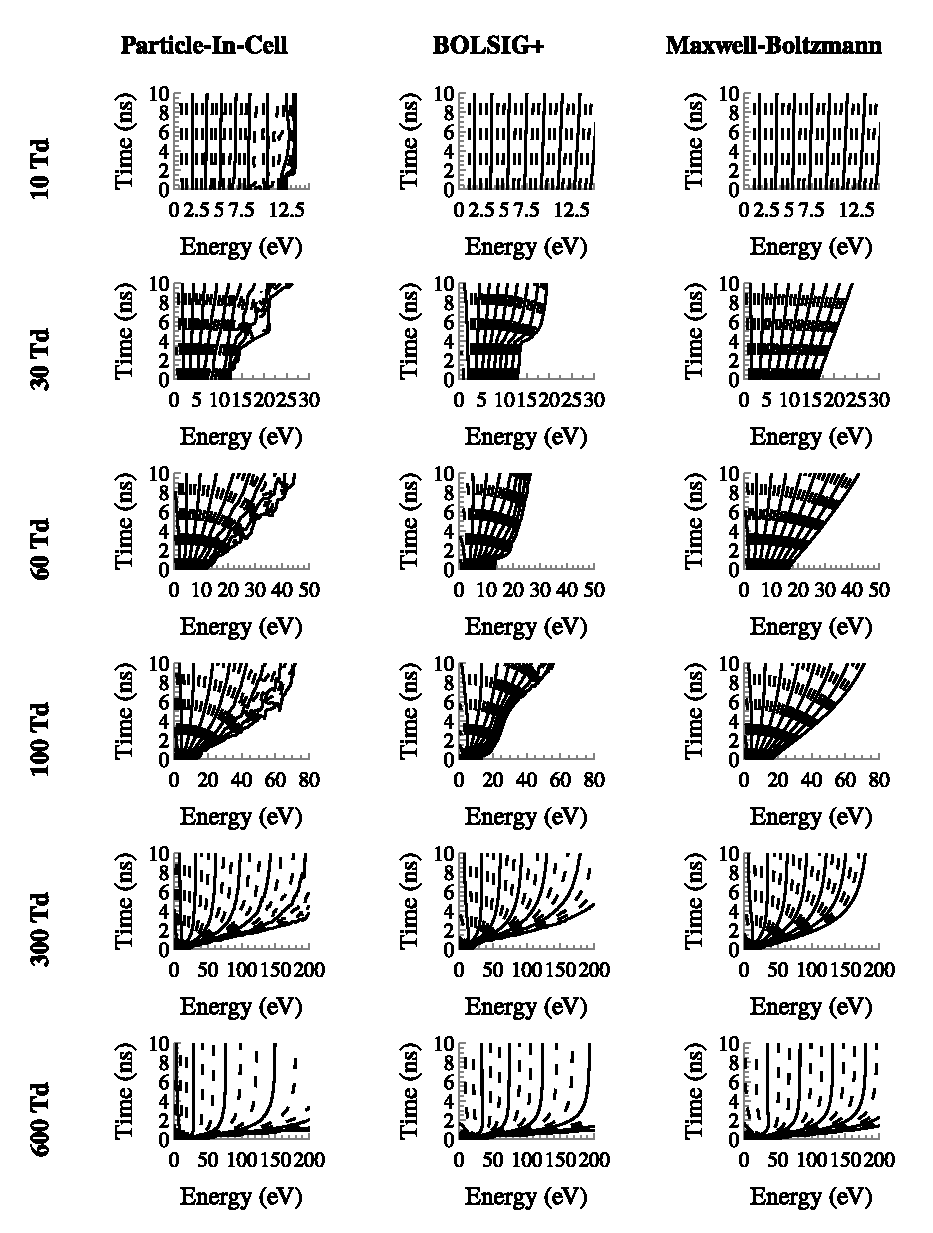
\includegraphics{./chapters/modeling/figures/picmb.eps}
  \caption{Contour plots of the \acs{eedf}s determined from \acs{pic}
    simulations, and the corresponding Maxwell-Boltmzann distributions for a range
    of electric fields.}
  \label{fig:picmb}
\end{figure}
as a series of contour plots on a logarithmic scale. The jaggedness of the
\acs{pic} simulations results from the finite number of particles in the system
and the low probability of high energy electrons. This problem is ameliorated at
higher electric fields where the probability of high-energy electrons increases.
It is also helped by the ionization processes which begin to occur after the
first few nanoseconds.

At 10 Td, the \acs{eedf}s are relatively unchanged over the duration of the
simulation. The subtle slopes of the contours suggest a small increase in the
overall temperature and energy of the system as a function of time. This is more
noticeable at 30 Td, where the contours have a more distinct slope. The spacing
between the slopes is relatively constant for each case--equivalent to a
Maxwell-Boltzmann distribution. However, there is some deviation at low energies
in the case of the BOLSIG+ solutions.

At 60 and 100 Td, the \acs{pic} results begin to exhibit contour spacings which
are consistent at low energies, but begin to grow at higher energies. This is
evidence of a growing population of high-energy electrons, in excess of what is
predicted by a Maxwell-Boltzmann distribution. Interestingly, the BOLSIG+
solutions exhibit unique contour shapes which are inconsistent with the other
cases. Additionally, the spacing of the contours is less consistent, with a
dearth of high energy electrons. 

By 300 and 600 Td this situation is reversed, as the Maxwell-Boltzmann
distributions begin to underestimate the population of high energy electrons.
Examination of the individual distributions shows that the \acs{pic} \acs{eedf}s
have a larger population of low energy (less than 20 eV) and high energy
(greater than 100 eV) electrons. This can be explained by the general shape of
the cross sections. The only reactions available to electrons in the \acs{pic}
simulations are elastic scattering, excitation (19.6 eV threshold), and
ionization (24.6 eV threshold). As the inelastic processes turn on at energies
in excess of the 20 eV, the electron population undergoes depletion. Likewise,
the electron population begins to rebound at higher energies as the cross
sections fall off.

Unlike Starikovskaia and Starikovskii's results \cite{Starikovskaia2001} the
various approaches produce comparable \acs{eedf}s. Generally, the
Maxwell-Boltzmann results provide the best match to the \acs{pic} simulations at
electric fields of 100 Td and below. Conversely, the BOLSIG+ results better
represent the \acs{eedf} past 100 eV at the higher field values. That said,
these electrons do not provide a large contribution to the excited states of the
plasma. They are well past the excitation and ionization cross section peaks and
are relatively few in number. Given the larger computational burden of the
Boltzmann solver and the small perceived benefit, it was concluded that the that
the Maxwell-Boltzmann distributions provided an adequate representation of
the \acs{eedf} for the global model.

\subsection{Energy Equation}

With an \acs{eedf} the rate coefficients in equation~\ref{eq:gcont} can be
calculated. However, as was seen in figure~\ref{fig:picmb}, the distribution
function changes over time. Previously, the \acs{pic} simulations were used to
determine the time evolution of the mean electron energy, but an alternate
approach was required for the global model.

With suitable assumptions, equation~\ref{eq:energy} (the second moment of the
Boltzmann equation) can provide the means by which the mean energy can be
evolved with each time step. Given the assumptions underlying the global model,
the spatial derivatives can be neglected such that
\begin{equation}
  \frac{d}{dt}\left(\frac{3}{2}p_e\right) =
  \frac{d}{dt}\left(\frac{3}{2}p_e\right)\bigg|_\mathrm{coll}.
\end{equation}
Using the isothermal equation of state \cite{Lieberman2005}, $p=n\kB T$, this
can be rewritten as,
\begin{equation}
  \frac{d}{dt}\left(\frac{3}{2}n_e\kB T_e \right) =
  \frac{d}{dt}\left(\frac{3}{2}n_e\kB T_e \right)\bigg|_\mathrm{coll}.
  \label{eq:energy2}
\end{equation}
The term on the RHS is the collision operator which expresses energy gained or
lost by electrons\footnote{In some plasmas, it is desirable to also treat gas
heating with a similar equation as it can have an appreciable impact on certain
rate constants. However, as noted in Chapter~\ref{chp:metastables}, the gas
temperature of the \acs{rpnd} in question remains at room temperature.} in
particle collisions.

Several different types of energy transfer were considered by the global model.
The first was the heating caused by the electric field. This was followed by
electron energy losses as a result of elastic scattering by the atoms. Finally,
inelastic collisions with all helium states through $n=4$ were considered.
Together, these phenomena replace the term on the RHS of
equation~\ref{eq:energy2} with,
\begin{equation}
  \frac{e^2n_eE(t)^2}{m_ek_m(T_e)N_g}
  - n_ek_m(T_e)N_g\left(\frac{3m_e}{M}\right)\frac{3}{2}\kB(T_e-T_g)
  - n_e \sum_i \sum_{j\neq i} K^e_{ij}N_i\Delta\epsilon_{ij},
  \label{eq:energyparts}
\end{equation}
where $E(t)$ is the time-varying electric field, $k_m$ is the electron momentum
transfer frequency from Pack et al. \cite{Pack1992}, and $\Delta\epsilon_{ij}$
is the energy lost or gained by the electron in atomic (de)excitation reactions.
The first term includes the DC conductivity \cite{Lieberman2005} of the plasma,
and accounts for the heating of the electrons by the electric field. The second
term is the elastic cooling of the electrons by the neutral atoms, where the gas
temperature. The third term is the energy gained or lost by the electrons in
atomic (de)excitation reactions. The
equations~\ref{eq:energyparts},~\ref{eq:energy2} and~\ref{eq:gcont} form the
primary components of the global model. Together they can be used to solve for
the evolution of the electron temperatures, electron densities, excited state
densities, and plasma emissions as functions of time.

\subsection{Model Solutions}

For the purposes of computation, equation~\ref{eq:gcont} can be rewritten for
each atomic state, $i$, resulting in a set of linear, first order differential
equations,
\begin{multline}
  \frac{d}{dt}
  \begin{pmatrix}
    N_1 \\
    N_2 \\
    \vdots \\
    N_M
  \end{pmatrix}
  = n_e
  \begin{pmatrix}
    -\sum_{j\neq 1}K^e_{1,j} & K^e_{2,1}      & \hdots & K^e_{M,1} \\
    K^e_{1,2}      & -\sum_{j\neq 2}K^e_{2,j} & \hdots & K^e_{M,2} \\
    \vdots         & \vdots         & \ddots & \vdots    \\
    K^e_{1,M}      & K^e_{2,M}      & \hdots & -\sum_{j\neq M}K^e_{M,j}
  \end{pmatrix}
  \cdot
  \begin{pmatrix}
    N_1 \\
    N_2 \\
    \vdots \\
    N_M
  \end{pmatrix} \\
  +
  \begin{pmatrix}
    0      & K^o_{2,1}              & \hdots & K^o_{M,1} \\
    0      & -\sum_{j < 2}K^e_{2,j} & \hdots & K^o_{M,2} \\
    \vdots & \vdots                 & \ddots & \vdots    \\
    0      & 0                      & \hdots & -\sum_{j < M}K^e_{M,j}
  \end{pmatrix}
  \cdot
  \begin{pmatrix}
    N_1 \\
    N_2 \\
    \vdots \\
    N_M
  \end{pmatrix} \\
  + N_g
  \begin{pmatrix}
    -\sum_{j\neq 1}K^a_{1,j} & K^a_{2,1}      & \hdots & K^a_{M,1} \\
    K^a_{1,2}      & -\sum_{j\neq 2}K^a_{2,j} & \hdots & K^a_{M,2} \\
    \vdots         & \vdots         & \ddots & \vdots    \\
    K^a_{1,M}      & K^a_{2,M}      & \hdots & -\sum_{j\neq M}K^a_{M,j}
  \end{pmatrix}
  \cdot
  \begin{pmatrix}
    N_1 \\
    N_2 \\
    \vdots \\
    N_M
  \end{pmatrix}, \\
\end{multline}
where $M$ is the total number of atomic states and $\epsilon_i <
\epsilon_{i+1}$. An additional equation can be added to separately account for
electrons as and electron-specific processes, however the global model used here
assumed quasineutrality by enforcing the relation $N_\mathrm{ion}=n_e$. Changes
in the density of each atomic state were calculated by numerical integration of
these equations. The range of time scales exhibited by the \acs{rpnd} made it
desirable to implement adaptive control of the time step size. For this reason,
the Runge-Kutta-Fehlberg method, adapted from Bradie \cite{Bradie2006}, was used
as the integration scheme.

The initial metastable densities came from the \acs{las} measurements while the
initial electron densities were determined from \acs{lcif} measurements made by
Weatherford \cite{Weatherford2012a}. Electron density measurements were only
available for 1.0, 4.0, and 8.0 Torr therefore, the global model analyses only
consider these conditions. Sensitivity to changes in the initial electron
density will be addressed in the following section.

It was necessary to assume a pre-pulse electron temperatures as no such
measurements were available. Given the relatively long period of time between
pulses, an in initial temperature of 0.2 eV was used. Exploratory simulations
found that changes in the initial electron temperature had a negligible impact
on the final distribution of excited states. Initial excited state densities
(not including ions and metastables) were determined from the 0.2 eV equilibrium
distribution of states. Per the results from Chapter~\ref{chp:metastables}, the
neutral gas temperature was fixed at 300 K for the duration of the simulation.

Despite access to the waveform of the applied potential, the actual
time-evolution of the electric field at the metastable measurement points is not
well known. This is a result of the distinctly nonlinear impedance of the
\acs{rpnd} plasma. Takashima et al.\ performed measurements of the electric
field in a \acs{fiw} using a capacitive probe and found it to be significantly
different from the vacuum field. Separately, Ito et al. \cite{Ito2010} and
M\"{u}ller et al. \cite{Muller2011a}, measured the electric fields in a
\acs{rpnd} with a 1.2 mm gap between parallel electrodes using a wave-mixing
approach. They too found a large difference between the vacuum field and the
actual field.

In all three cases, the evolution of the electric field could be best described
by a Gaussian-like pulse, followed by a small, persistent electric field. This
persistent field was on the order of 20-25\% of the peak field value, and would
remain for at least several tens of nanoseconds. The total duration and
magnitude of the persistent field varied between studies and some, such as the
work of Anikin et al. \cite{Anikin1998}, did not find evidence of it. Given the
uncertainty associated with the nature of this persistent field, the global
model simulations only considered a single Gaussian pulse. The time domain of
the simulations covered 190 ns with the peak of the pulse centered at 40 ns.

\section{Perturbation Study}

The input values for the initial metastable density, electron density, and
pressure were fixed. However, the same could not be said for the peak electric
field and the width of the pulse. It was initially expected that the pulse-width
would be approximately equal to the width of the applied pulse, 25 ns. The
global models were matched to the metastable measurements by iterative
adjustment of the peak electric field and the pulse-width. However, there was no
clear means by which to estimate the error in the global model calculations.

In order to provide a qualitative understanding of the possible error, a
preliminary fit of the 4.0 Torr data was made and used as a benchmark.
Subsequent simulations were run with small perturbations to the peak electric
field, pressure, pulse-width, and initial electron density. In each case, the
benchmark value was perturbed by $\pm10\%$.

The nominal conditions of the simulation are recorded in table~\ref{tbl:nominal}
\begin{table}
  \centering
  \caption{Nominal simulation parameters for the 4.0 Torr operating condition.}
  \begin{tabular}{llll}
    \toprule
    Pressure & Initial Electron    & Pulse      & Peak Electric \\
    (Torr)   & Density (m$^{-3}$)  & width (ns) & Field (Td)\\ 
    \midrule
    4.0      & 5.36$\times10^{13}$ & 40         & 207 \\
    \bottomrule
  \end{tabular}
  \label{tbl:nominal}
\end{table}
and results of these simulations are shown in figure~\ref{fig:perturbed}.
\begin{figure}
  \centering
  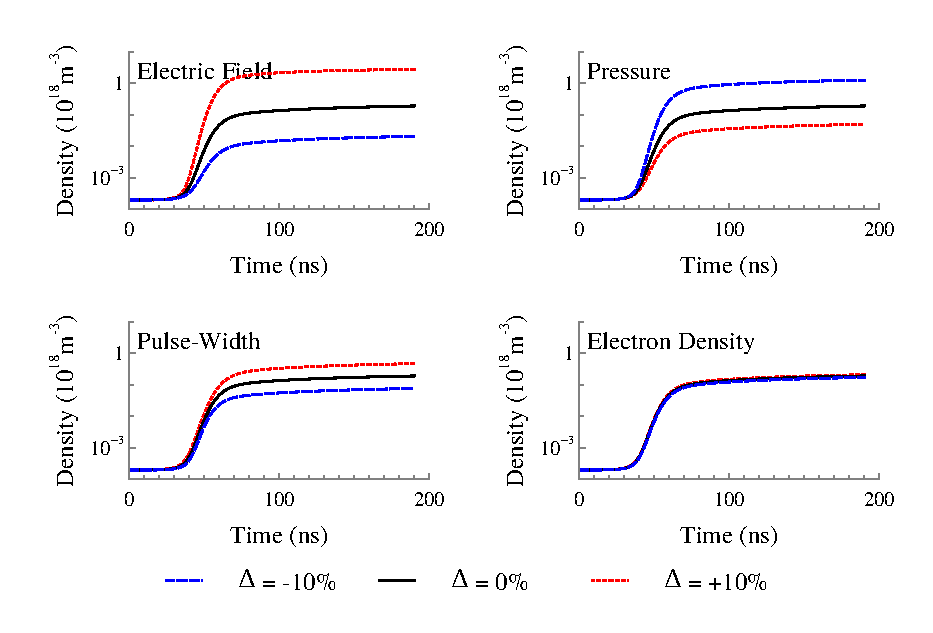
\includegraphics{./chapters/modeling/figures/perturbed.eps}
  \caption{Simulations showing the effects of perturbations to the initial
  conditions on the metastable dynamics.}
  \label{fig:perturbed}
\end{figure}
The metastable trends suggest that the initial electron density has a relatively
small impact on the metastable dynamics. Closer examination reveals that the
final metastable densities change by approximately $\pm10\%$, almost one-to-one
with the initial electron density. In contrast, changes to the pulse-width
produce much more significant changes in the metastable densities. As the
pulse-width is increased, the metastable densities increase. As the electric
field was fixed for these simulations, this change can be attributed to the
increase in energy deposited in the electron population.

The two most influential factors in the determination of the metastable
densities were the neutral gas pressure and the electric field. The
perturbations to these quantities resulted in largest changes in the final
metastable densities. As can be seen in figure~\ref{fig:perturbed}, increases in
pressure corresponded to a decrease in metastable densities. Changes to the
neutral gas pressure tend to affect the system via several different mechanisms.
As seen in equation~\ref{eq:energyparts}, increases to the gas pressure tend to
decrease the energy deposited in the electrons, and increases losses due to
elastic scattering. This reduces the energy that can be deposited in excited
states. However, the reduced electron energy density competes with the increased
number of ground state atoms available for excitation. The perturbation results
indicate that the reduced energy deposition in the electrons is more significant
than the increased availability of neutral atoms.

The large influence of the electric field can be traced back to changes in the
ionization rate for each condition. As seen in figure~\ref{fig:ionrates},
\begin{figure}
  \centering
  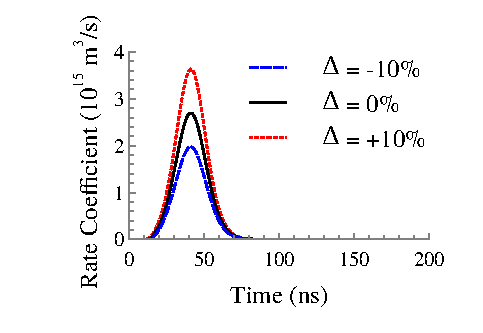
\includegraphics{./chapters/modeling/figures/ionrates.eps}
  \caption{Ionization rates coefficients corresponding to the perturbed electric
  field simulations.}
  \label{fig:ionrates}
\end{figure}
the magnitude of the ionization rate coefficient corresponds to the magnitude of
the electric field. While the changes are somewhat modest, as seen in
Chapter~\ref{chp:theory}, ionization processes exponentially with time. This
means that small changes to the rate coefficient manifest as large differences
in the final electron density. Since the rate of metastable generation is
proportional to the electron density, large changes to the electron density
equate to large changes in the metastable density.

\section{Plasma Dynamics}

The plasma dynamics for the 1.0, 4.0, and 8.0 Torr conditions were obtained by
iteratively matching the pulse-width and peak electric field to the metastable
density immediately before the arrival of the reflected pulse. The process was
somewhat complicated by the fact that multiple combinations of the peak field
and pulse-width could produce the same metastable density. Therefore, it was
necessary to fix or otherwise predict one of the values.

Of the two, the pulse-width was the most promising to eliminate as a variable.
The characteristics of the applied pulse already provided a bound on the
possible widths. Therefore, the 4.0 Torr condition was simulated with a range of
pulse-widths from 5-50 ns with the peak field selected to produce the same final
metastable density in each case.

The metastable density trend for each pulse-width is compiled in
figure~\ref{fig:widths}.
\begin{figure}
  \centering
  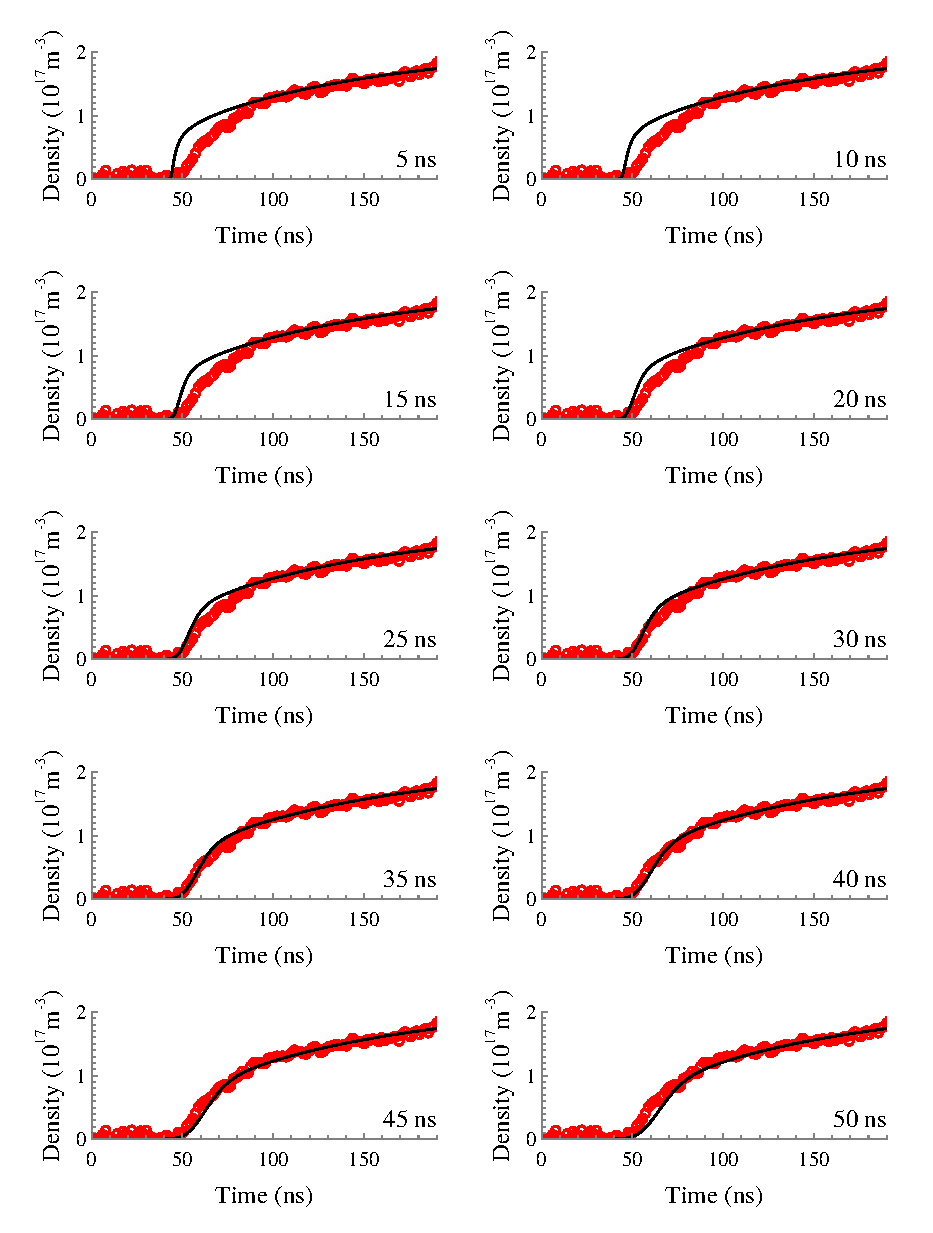
\includegraphics{./chapters/modeling/figures/widths.eps}
  \caption{Comparison of measured metastable values (represented by open
    circles) to simulations with a range of pulse-widths.}
  \label{fig:widths}
\end{figure}
It is immediately apparent that the short pulse-widths do not provide an optimal
description of the data. This includes the results for the 25 ns simulation
which shows a much high production rate of metastables than was observed in the
experiment. The time resolution of the experimental measurements was determined
by the photodiode which had a response time of 5 ns. Therefore, the slowed
change in metastable density appears to be a real phenomena. This suggested that
the effective pulse-width in the \acs{rpnd} extended longer than the duration of
the applied voltage. Indeed, the best match of the data for the illustrated
simulations occurs for a pulse-width of 40 ns.

The results of the pulse-width comparison suggested that additional excitation
was taking place beyond the applied pulse. In order to determine the origin of
this excitation, a survey was made of the neutral emissions spectra. The details
of these measurements will be discussed in more detail in
Chapter~\ref{chp:emissions}. The emissions for each transition were expected to
follow the same basic trend: an initial rise correlating with the voltage pulse,
followed by a monotonic decay. However, several transitions exhibited trends
that differed from this. The evolution of the 4$^1$P$^\mathrm{o}$-2$^1$S
transition at 396 nm was a good example of this deviation and is reproduced in
figure~\ref{fig:double}.
\begin{figure}
  \centering
  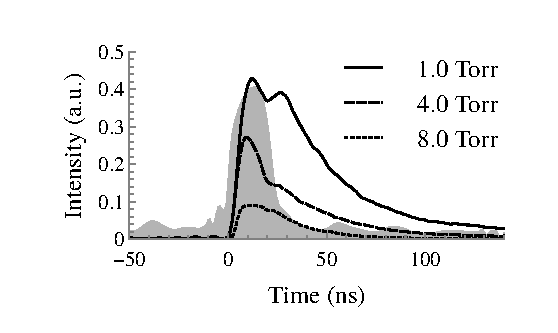
\includegraphics{./chapters/modeling/figures/double.eps}
  \caption{The emissions of the 4$^1$P$^\mathrm{o}$-2$^1$S transition in the
  \acs{rpnd}, overlaid on top of the voltage pulse.}
  \label{fig:double}
\end{figure}
Here the emissions for each operating condition have been overlaid on the
applied voltage pulse for comparison. The voltage pulse clearly coincides with
an initial increase in the number of helium atoms occupying the
4$^1$P$^\mathrm{o}$ state. 15 ns later, another increase is visible,
particularly at 1.0 and 4.0 Torr. This second transient is similar to the return
strokes observed in streamer research \cite{Snoddy1936, Loeb1940, Mitchell1947}.
The observation of return strokes in similar studies \cite{Vasilyak1994,
Pai2009, Starikovskiy2013} suggests that this is a reasonable explanation for
the double-peaked emissions. If the forward and return strokes possess durations
equal to the applied voltage (25 ns), separated by 15 ns, then the excitation
period would be approximately 40 ns. This is consistent with the pulse-width
required to match the observed data. As a result, a pulse-width of 40 ns was
used in all subsequent simulations.

Figure~\ref{fig:fieldtau}
\begin{figure}
  \centering
  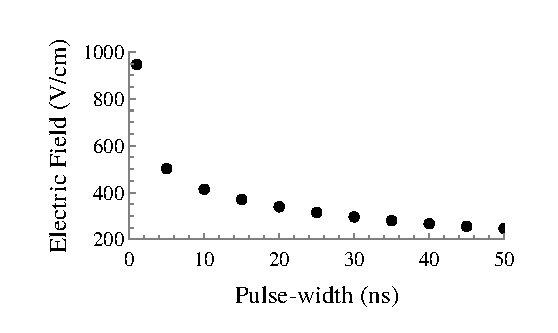
\includegraphics{./chapters/modeling/figures/fieldtau.eps}
  \caption{The electric fields necessary to generate the same metastable density
    at 4.0 Torr as a function of the pulse-width.}
  \label{fig:fieldtau}
\end{figure}
is a scatter plot of the peak electric fields necessary to obtain the same final
metastable density as a function of the pulse-width. Initially, as the
pulse-width is decreased from 50 ns, only small increases of the electric field
are required to obtain the same number of metastable atoms. However, as the
pulse-width is decreased further, the rate at which the electric field must
increased grows substantially.

Eventually, for short enough pulses, it is no longer possible to maintain the
same metastable density, regardless of further increases in the electric field.
This occurs for the same reason that the \acs{eedf} from the \acs{pic}
simulations was depressed between 20 and 100 eV--eventually, the cross sections
fall off with increasing electron energy. This places an upper limit on the rate
coefficient as a function of electron temperature and a limit to the number of
metastables which can be generated in a given period of time.
Figure~\ref{fig:longrates}
\begin{figure}
  \centering
  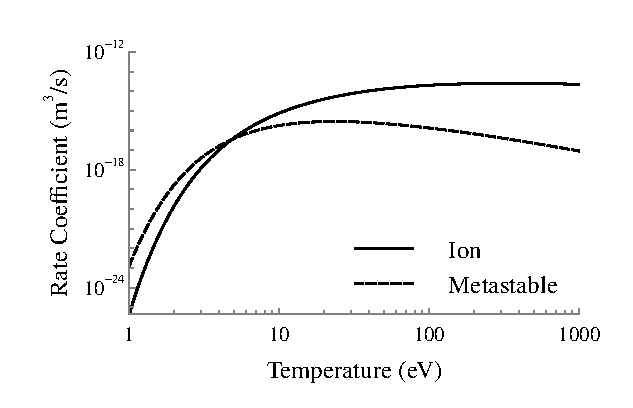
\includegraphics{./chapters/modeling/figures/longrates.eps}
  \caption{Ionization and metastable rate coefficients as functions of
    electron temperature.}
  \label{fig:longrates}
\end{figure}
shows the ionization and metastable rate coefficients as functions of the
electron temperatures in the system. The ionization rate coefficient peaks at
approximately 320 eV, while the metastable rate coefficient peaks much lower at
around 23 eV. These rate coefficients, along with the general form of the cross
sections for the reactions, show that there is an optimal field strength for
ionization and excited state generation. Further increases in the electric field
would only serve to reduce to reduce the final density of these particles.
However, there may be additional benefits in the use of a higher electric field.
The runaway electrons which can be generated at these field strengths, described
by Vasilyak \cite{Vasilyak1994} among others, could help increase the discharge
volume and homogeneity via nonlocal energy deposition.

Figure~\ref{fig:nmcomp}
\begin{figure}
  \centering
  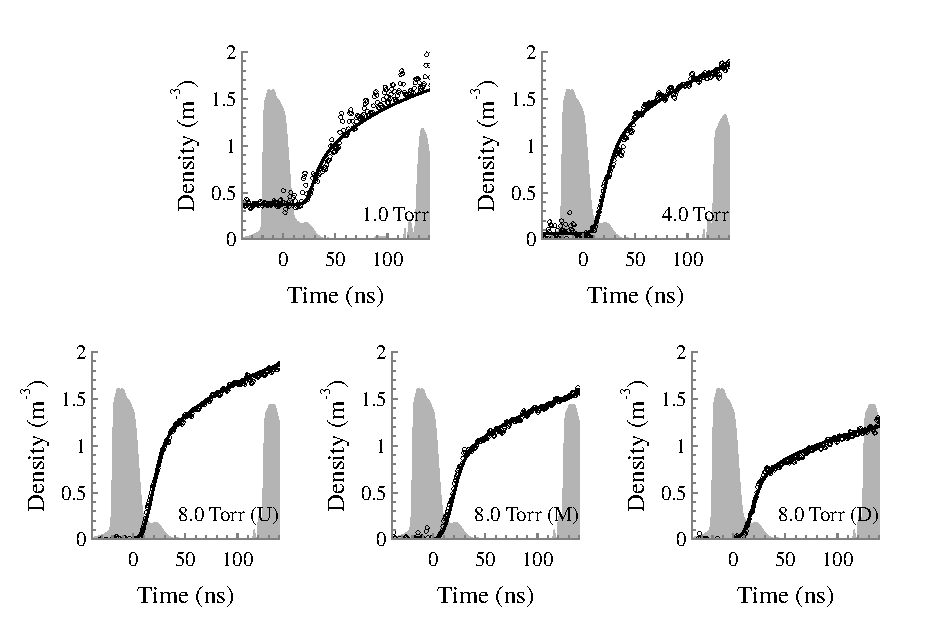
\includegraphics{./chapters/modeling/figures/nmcomp.eps}
  \caption{Comparison of the measured metastable densities (open circles) to
    the global model simulations. The shaded region illustrates the applied
    voltage pulse. The parentheses following the 8.0 Torr labels indicate the
    axial location of the measurement.}
  \label{fig:nmcomp}
\end{figure}
shows the comparison of the measured metastable densities for 1.0, 4.0, and 8.0
Torr overlaid atop the applied voltage pulse\footnote{The relative timing of the
metastable measurements and the voltage pulse are approximate. Corrections were
made in post-processing to account for different cable lengths in the system.}.
As seen in chapter~\ref{chp:metastables}, there was little axial variation in
the metastable measurements at 1.0 and 4.0 Torr. For this reason, simulations
were conducted only for the measurements at the midstream positions. In
contrast, the axial distribution of metastables showed noticeable variation at
8.0 Torr. Therefore, each location was considered independently in the
simulations.

Despite the assumptions involved in the development of the global model, the
simulation results show impressive agreement with the measurements. This
includes the period of 0-40 ns when the metastable growth rate is the largest.
The plasma behavior during this time is dominated by energetic electrons that
have been accelerated by the large electric fields. Given the relatively short
period, inter-atomic and radiative processes play a relatively unimportant role.
The most significant discrepancies appear in the 1.0 Torr simulations where the
global appears to overestimate the metastable density during the pulse.

The global model also performs well in the afterglow period, from 40 ns to the
end of the measurements. After the pulse, the electrons begin to undergo rapid
cooling, as seen in figure~\ref{fig:etemps}.
\begin{figure}
  \centering
  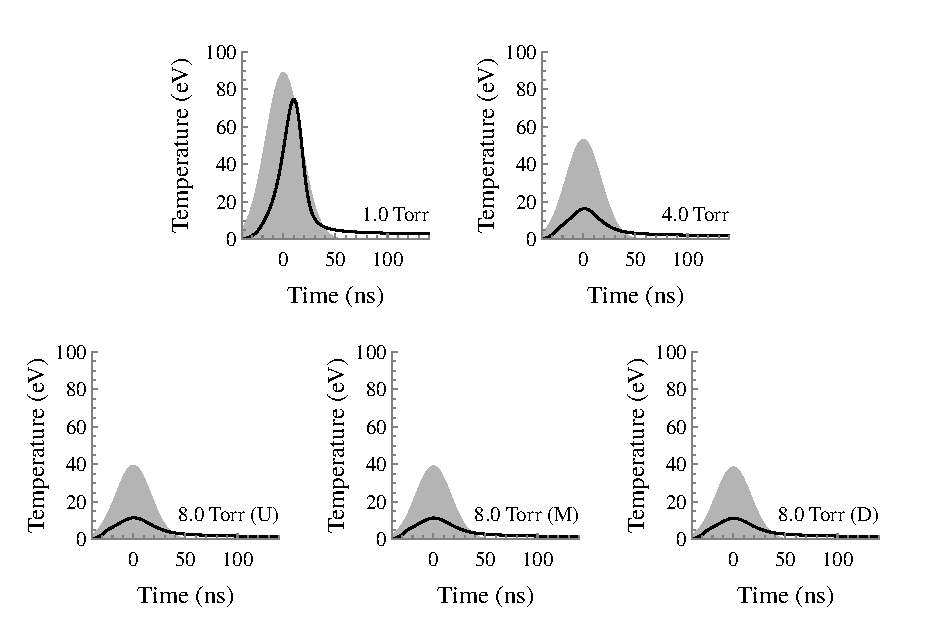
\includegraphics{./chapters/modeling/figures/etemps.eps}
  \caption{Global model predictions of the electron temperatures at the
  simulated conditions, overlaid on the corresponding electric field.}
  \label{fig:etemps}
\end{figure}
By 50 ns, the electron temperatures have fallen below 10 eV in all cases, and by
the end of the simulation they are all below 3 eV. As a result of this rapid
cooling, the rate of electron-induced reactions falls significantly. As was seen
in figure~\ref{fig:longrates}, the rate for metastable and ion generation begin
to undergo a fast decline at temperatures below 10 eV. This indicates that much
of the metastable growth after 50 ns can be attributed to downward radiative
transitions from upper excited states. Again, the most significant discrepancies
appear for the measurements at 1.0 Torr. In this case, the simulations appear to
underestimate the total metastable population.

The issues in accurately simulating the 1.0 Torr case may be a result of the
large electric field present in the system. As can be observe in
table~\ref{tbl:simsum}
\begin{table}
  \centering
  \caption{Summary of the peak values for several plasma parameters from the
  global model simulations.}
  \begin{tabular}{lllll}
    \toprule \\
    Pressure         & E/N  & T$_\mathrm{e}$ & N$_\mathrm{m}$ & n$_\mathrm{e}$ \\
    (Torr)           & (Td) & (eV)           &  (m$^{-3}$)    & (m$^{-3}$) \\
    \midrule \\
    1.0              & 346  & 74.6           & 1.62$\times10^{17}$ & 
      5.17$\times10^{17}$ \\
    4.0              & 207  & 16.3           & 1.87$\times10^{17}$ &
      3.41$\times10^{17}$ \\
    8.0 (Upstream)   & 154  & 11.5           & 1.88$\times10^{17}$ &
      2.60$\times10^{17}$ \\
    8.0 (Midstream)  & 152  & 11.4           & 1.57$\times10^{17}$ & 
      2.16$\times10^{17}$ \\
    8.0 (Downstream) & 150  & 11.3           & 1.21$\times10^{17}$ &
      1.67$\times10^{17}$ \\
    \bottomrule
  \end{tabular}
  \label{tbl:simsum}
\end{table}
the electric field approaches 350 Td for the 1.0 Torr discharge. This
corresponds to the regime in which the Maxwell-Boltzmann distribution (as well
as the BOLSIG+ results) begin to deviate from the \acs{pic} predictions.
Specifically, the Maxwell-Boltzmann distribution tended to overestimate the
number of electron in the range of 20-100 eV at high electric fields. These are
precisely the electrons which are responsible for the generation of the
metastable states. This suggests that the assumption of a Maxwell-Boltzmann
distribution would tend to overestimate the metastable generation at large
electric fields, consistent with what is observed in figure~\ref{fig:nmcomp}.

As the global model is applied to increasing pressures, the reduced electric
field begins to fall. Likewise, the electron temperatures are also reduced, from
about 75 eV down to 12 eV. Despite these changes, the final metastable densities
remain approximately the same. Though the temperatures are lower, they still
peak near the maximum in the metastable rate coefficient in
figure~\ref{fig:longrates}. Additionally, the large number of neutral gas
particles ensures that the total metastable production rate remains large.

Notably, the metastable densities and electron densities peak for different
conditions. The electron density trends can be observed in
figure~\ref{fig:necomp}
\begin{figure}
  \centering
  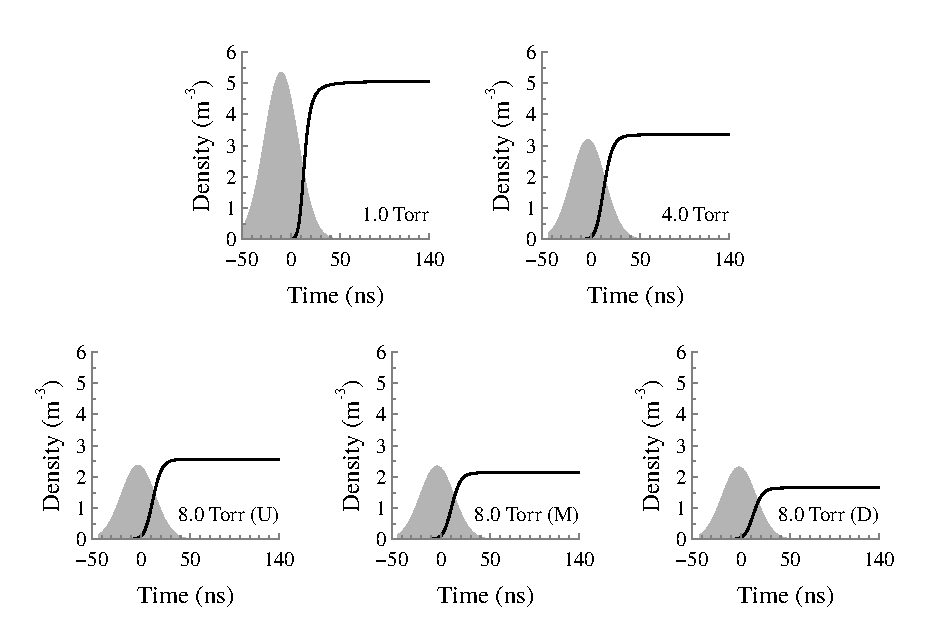
\includegraphics{./chapters/modeling/figures/necomp.eps}
  \caption{Global model predictions of the electrons densities at the simulated
  conditions overlaid on the reduced electric field.}
  \label{fig:necomp}
\end{figure}
overlaid on the reduced electric fields. The electron density peaks at the
lowest simulated pressure whereas the metastable density peaks at 4.0 Torr.
Again, this can be seen as a result of the rate coefficients for the respective
reactions. The ionization rate coefficient continues to increase well past 100
eV, whereas the metastable rate coefficient decreases after 23 eV. While the
increase in electron density competes with the decline in the metastable rate
coefficient, ultimately the rate coefficient falls too quickly. 

Also observable in the evolution of the electron densities is a time-delay
between the peak electric field and peak electron production rate for all
conditions. For the cases under consideration the peak ionization rate occurs at
about 23.5 ns at 1.0 Torr, 16.4 ns at 4.0 Torr, and 15.5 ns at 8.0 Torr. In
contrast, the electron temperatures in figure~\ref{fig:etemps} show little to no
such delay. In part, this behavior reflects the need for a finite amount of time
before the background electrons gain ionization-relevant energies. Additionally,
the electron growth process is relatively slow at first given the low initial
densities. This explanation is consistent with the initial electron densities
measured by Weatherford \cite{Weatherford2012a} which showed the largest
pre-pulse density at 8.0 Torr, and the smallest at 1.0 Torr.

Finally, the behavior axial behavior in the 8.0 Torr condition exhibits several
interesting characteristics. At the position closest to the anode, the peak
metastable density exceeds that of operation at 4.0 Torr. This contrasts with
the position furthest from the anode which features the lowest measured
metastable density for this range of conditions. However, the electric field and
electron temperatures across all three locations only vary by about one percent.
This recalls the electric field sensitivity that was noted in the earlier
perturbation study and suggests that even small variations in the electric field
of the \acs{rpnd} can have large implications on its homogeneity.

\section{Summary}

The metastable density measurements were only able to provide limited insight on
the development of the \acs{rpnd}. However, production of the metastable atoms
is determined by a number of other plasma quantities such as electron
temperature, density, and electric field strength. Following a series of
assumptions, a global model simulation was developed in order to infer the
dynamics of these other quantities. The development of the model carefully
considered the choice of distribution function and the sensitivity to various
initial conditions.

A comparison of several preliminary simulations to measured metastable data
indicated the need for an electric field with a duration longer than applied
voltage pulse. Examination of the plasma emissions showed that the extended
excitation could be attributed to a return stroke in the system. Use of this
extended excitation time yielded excellent agreement for all but the 1.0 Torr
condition. In this case, what appeared to be mild deviations appeared with the
model overestimating metastable production rate during the pulse, and
underestimating it afterward. Given the large electric fields in this condition,
these discrepancies can most likely be attributed to differences between the
assumed \acs{eedf} and those in the actual device.

It was found that breakdown of the \acs{rpnd} was accompanied by a finite delay
between the peak electric field value and the peak ionization rate. As the
generation of electrons is essentially exponential, this appeared to be the
result of the low pre-pulse electron densities and the finite heating time.
Interestingly, the peak electron and metastable densities did not coincide.
Instead, highest predicted electron density occurred at the same condition as
optimal energy coupling to the plasma, as seen in Chapter~\ref{chp:experiment}.
Simultaneously, as will be seen in Chapter~\ref{chp:emissions}, the peak
metastable density is associated with the peak brightness of the plasma, the
largest number of excited states, and the highest wave velocity. These
contrasting results demonstrate that the \acs{rpnd} can be optimized for one of
two conditions: production of excited atomic states, or ionization.
